\documentclass{article}
\title{Intro to PDEs: Ch 2.3 HW}
\author{Logan Rhyne, Harley Combest, Roy Galang, Jesse DiCenso}
\usepackage[T1]{fontenc}
\usepackage{amsfonts, amsmath, amsthm, amssymb}
\usepackage{mathtools, bigints, empheq}
\usepackage{graphicx, wrapfig, xcolor, float}
\usepackage{stackrel}
\usepackage{pgfplots}
\usepackage[shortlabels]{enumitem}
\usepackage[margin=1.0in]{geometry}
\setlength{\parindent}{0pt}
\theoremstyle{definition}
\newtheorem*{lemma}{Lemma}
\newtheorem*{conj}{Conjecture}
\newtheorem{prob}{}
\newtheorem*{pf}{Proof}
\newtheorem*{dpf}{Disproof}
\renewcommand\qedsymbol{$\blacksquare$}
\renewcommand{\emptyset}{\varnothing}
\renewcommand{\epsilon}{\varepsilon}
\newenvironment{disproof}{\begin{proof}[Disproof]}{\end{proof}}
\newenvironment{ans}{\begin{proof}[Answer]\renewcommand{\qedsymbol}{}}{\end{proof}}
\newenvironment{boldenv}{\bfseries\boldmath}{}
\newcommand{\N}{\mathbb{N}}
\newcommand{\Z}{\mathbb{Z}}
\newcommand{\R}{\mathbb{R}}

\pgfplotsset{compat=1.18}

\DeclareMathOperator{\ran}{range}
\DeclareMathOperator{\sech}{sech}

\begin{document}

    \maketitle

\begin{boldenv}
    \underline{Problem 1}. Find the general solutions of
    \begin{enumerate}[(1), series=problems]
        \item $u_{tt} - u_{xx} = 0$
        \item $u_{tt} - 4u_{xx} = 0$
        \item $u_{tt} - 9u_{xx} = 0$
        \item $4u_{tt} - u_{xx} = 0$
        \item $4u_{tt} - 9u_{xx} = 0$
    \end{enumerate}
\end{boldenv}
\begin{ans}
\begin{enumerate}[(1), series=answers]
    \item A general wave equation takes the form $u_{tt}-c^2u_{xx} = 0$, and its solution is $u(t,x) = f(x+ct) + g(x-ct)$. As the equation shows, $c^2 = 1$, so the general solution of this wave equation is
    \[\boxed{u(t,x) = f(x+t) + g(x-t)}\].
    \item The general solution of the wave equation is given by
    \[u(t,x) = f(x-ct) + g(x+ct).\]
    We may easily conclude based on the form of the wave equation itself that $c = 2$. Therefore, the general solution is
    \[\boxed{u(t,x) = f(x-2t) + g(x+2t)}.\]
    \item From the general solution of the wave equation and $c^2 = 9$ we have\\ 
    \[\boxed{u(t, x) = f(x + ct) + g(x-ct) =- f(x+3t) + g(x-3t)}\] \\
    as our solution to the wave equation.
    \item Dividing both sides by $4$ yields
    $$u_{tt}-\frac{1}{4}u_{xx}=0$$
    It is clear that this is a wave equation with $c=\frac{1}{2}$, to which the general solution is
    \[\boxed{u(t,x) = f\left(x-\frac{1}{2}t\right)+g\left(x+\frac{1}{2}t\right)}\]
    \item Dividing both sides by 4 yields
    \[ u_{tt} - \frac{9}{4}u_{xx} = 0 \]
    In other words, $c = \frac{3}{2}$, and the solution to the wave equation is
    \[\boxed{u(t,x)=f\left(x+\frac{3}{2}t\right) + g\left(x-\frac{3}{2}t\right)}\]
\end{enumerate}
\end{ans}

For the next problem, the following diagrams will be referred to in the discussion:\\
Diagram 1:
\begin{center}
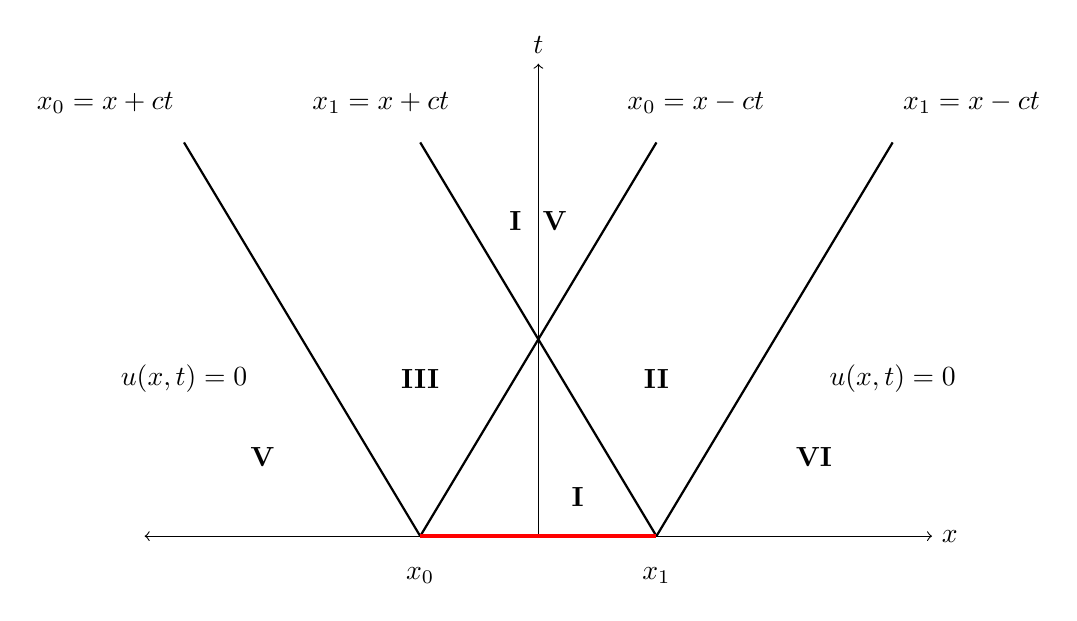
\begin{tikzpicture}[scale=0.5]
\draw[<->] (-10,0) -- (10,0) node[right] {$x$};
\draw[->] (0,0) -- (0,12) node[above] {$t$};

\draw [black, thick] (3, 0) -- ++(6 , 10);
\draw [black, thick] (3, 0) -- ++(-6 , 10);
\draw [black, thick] (-3, 0) -- ++(6 , 10);
\draw [black, thick] (-3, 0) -- ++(-6 , 10);
\draw [red, ultra thick] (-3,0) -- (3,0);

\node at (1, 1) {\textbf{I}};
\node at (3, 4) {\textbf{II}};
\node at (-3, 4) {\textbf{III}};
\node at (0, 8) {\textbf{I \ V}};
\node at (-7, 2) {\textbf{V}};
\node at (7, 2) {\textbf{VI}};

\node at (3, -1) {$x_1$};
\node at (-3, -1) {$x_0$};
\node at (-4 , 11) {\textbf{$x_1 =x + ct$}};
\node at (-11 , 11) {\textbf{$x_0 =x + ct$}};
\node at (4 , 11) {\textbf{$x_0=x - ct$}};
\node at (11 , 11) {\textbf{$x_1 = x - ct$}};
\node at (-9, 4) {\textbf{$u(x,t) = 0$}};
\node at (9, 4) {\textbf{$u(x,t) = 0$}};

\end{tikzpicture}
\end{center}

Diagram 2:
\begin{center}
\begin{tikzpicture}[scale=0.5]
\draw[<->] (-10,0) -- (10,0) node[right] {$x$};
\draw[->] (0,0) -- (0,12) node[above] {$t$};

\draw [black, thick] (0, 0) -- ++(6 , 10);
\draw [black, thick] (0, 0) -- ++(-6 , 10);

\node at (5, 5) {\textbf{I}};
\node at (0, 8) {\textbf{I \ I}};
\node at (-5, 5) {\textbf{III}};

\node at (-6 , 11) {\textbf{$x=-ct$}};
\node at (6 , 11) {\textbf{$x=ct$}};
% \node at (-9, 4) {\textbf{$u(x,t) = 0$}};
% \node at (9, 4) {\textbf{$u(x,t) = 0$}};

\end{tikzpicture}
\end{center}

\begin{boldenv}
    \underline{Problem 2}. Solve IVP
        \[\begin{cases}
        u_{tt} - c^2u_{xx} = 0\\
        u|_{t=0}=g(x), u_t|_{t=0} = h(x)
    \end{cases}\]
    with \begin{enumerate}[start=7, resume*=problems]
        \item \begin{equation*}
        g(x) =
        \begin{cases}
            0, x<0\\
            1, x\geq0
        \end{cases}
        \end{equation*}
        \[h(x) = 0\]
        
        \item \begin{equation*}
        g(x) =
        \begin{cases}
            1, |x|<1\\
            0, |x|\geq1
        \end{cases}
        \end{equation*}
        \[h(x) = 0\]
        
        \item \begin{equation*}
        g(x) =
        \begin{cases}
            1-|x|, |x|<1\\
            0, |x|\geq1
        \end{cases}
        \end{equation*}
        \[h(x) = 0\]
        
        
        \item \begin{equation*}
        g(x) =
        \begin{cases}
            1-x^2, |x|<1\\
            0, |x|\geq1
        \end{cases}
        \end{equation*}
        \[h(x) = 0\]
        
        \item \begin{equation*}
        g(x) =
        \begin{cases}
            \cos{(x)}, |x|<\frac{\pi}{2}\\
            0, |x|\geq\frac{\pi}{2}
        \end{cases}
        \end{equation*}
        \[h(x) = 0\]
        
        \item \begin{equation*}
        g(x) =
        \begin{cases}
            \cos^2{(x)}, |x|<\frac{\pi}{2}\\
            0, |x|\geq\frac{\pi}{2}
        \end{cases}
        \end{equation*}
        \[h(x) = 0\]
        
        \item \begin{equation*}
        g(x) =
        \begin{cases}
            \sin{(x)}, |x|<\pi\\
            0, |x|\geq\pi
        \end{cases}
        \end{equation*}
        \[h(x) = 0\]
        
        \item \begin{equation*}
        g(x) =
        \begin{cases}
            \sin^2{(x)}, |x|<\pi\\
            0, |x|\geq\pi
        \end{cases}
        \end{equation*}
        \[h(x) = 0\]
        
        \item
        \[g(x) = 0\] \begin{equation*}
        h(x) =
        \begin{cases}
            0, x<0\\
            1, x\geq0
        \end{cases}
        \end{equation*}
        
        \item
        \[g(x) = 0\] \begin{equation*}
        h(x) =
        \begin{cases}
            1-x^2, |x|<1\\
            0, |x|\geq0
        \end{cases}
        \end{equation*}
        
        \item
        \[g(x) = 0\] \begin{equation*}
        h(x) =
        \begin{cases}
            1, |x|<1\\
            0, |x|\geq1
        \end{cases}
        \end{equation*}
        
        \item
        \[g(x) = 0\] \begin{equation*}
        h(x) =
        \begin{cases}
            \cos{(x)}, |x|<\frac{\pi}{2}\\
            0, |x|\geq\frac{\pi}{2}
        \end{cases}
        \end{equation*}
        
        \item
        \[g(x) = 0\] \begin{equation*}
        h(x) =
        \begin{cases}
            \sin{(x)}, |x|<\pi\\
            0, |x|\geq\pi
        \end{cases}
        \end{equation*}
    \end{enumerate}
\end{boldenv}

\begin{ans}
\begin{enumerate}[(1), start = 7, resume*=answers]
    \item For these problems, we will use D'Alembert's formula, the solution to the wave equation. This formula is
    \[u(x,t) = \frac{1}{2}(g(x+ct) + g(x-ct)) + \int_{x-ct}^{x+ct}h(s)ds\]
    For this problem, we have $h(x)=0$; this means we don't use the integral term of D'Alembert's formula. We have that $x_0=-1$ and $x_1=1$. Taking a point in each of the regions in diagram 2 yields
    
      \[\boxed{u(x,t) = \begin{cases}
        1 & (x,t)\in \text{Region I}\\
        \frac{1}{2} & (x,t)\in \text{Region II}\\
        0 & (x,t)\in \text{Region III}
    \end{cases}}\]


    \item Since $h(x) = 0$, we don't have to worry about the integral term of D'Alembert's formula. For this problem, we have $x_0 = -1$ and $x_1 = 1$. Taking a point $(\Tilde{x}, \Tilde{t})$ in each region of diagram 1 and tracing it down to the points $(0, \Tilde{x} + c\Tilde{t})$ and $(0, \Tilde{x} - c\Tilde{t})$ lets us know that the solution is given by the following:
    \[\boxed{u(x,t) = \begin{cases}
        1 & (x,t)\in \text{Region I}\\
        \frac{1}{2} & (x,t)\in \text{Region II and III}\\
        0 & (x,t)\in \text{Region IV, V, and VI}
    \end{cases}}\]

    \item 
        Since $h(x) = 0$, we don't have to worry about the integral term of D'Alembert's formula. For this problem, we have $x_0 = -1$ and $x_1 = 1$. Taking a point $(\Tilde{x}, \Tilde{t})$ in each region of diagram 1 and tracing it down to the points $(0, \Tilde{x} + c\Tilde{t})$ and $(0, \Tilde{x} - c\Tilde{t})$ lets us know that the solution is given by the following:
        \[\boxed{u(x,t) = \begin{cases}
        \frac{1}{2} \left[ 1-|x+ct| + 1-|x-ct| \right]\ & (x,t)\in\text{Region I}\\
        \frac{1}{2} \left[ 1-|x-ct| \right] & (x,t)\in\text{Region II}\\
        \frac{1}{2} \left[ 1-|x+ct| \right] & (x,t) \in \text{Region III}\\
        0 & (x,t) \in \text{Region IV, V, and VI}
    \end{cases}}\]

    \item With D'Alembert's formula, we can see that $h(x) = 0$, so we use diagram 1 with $x_0 = -1$ and $x_1 = 1$. This means the possible solutions to the wave equation are:
    \[\boxed{u(x,t) = \begin{cases}
        \frac{1}{2} \left[ 1-(x+ct)^2 + 1-(x-ct)^2 \right]\ & (x,t)\in\text{Region I}\\
        \frac{1}{2} \left[ 1-(x-ct)^2 \right] & (x,t)\in\text{Region II}\\
        \frac{1}{2} \left[ 1-(x+ct)^2 \right] & (x,t) \in \text{Region III}\\
        0 & (x,t) \in \text{Region IV, V, and VI}
    \end{cases}}\]
    
    \item As $h(x) = 0$, we utilize diagram 1 with $x_0 = -\frac{\pi}{2}$ and $x_1 = \frac{\pi}{2}$ to find our solutions, which are
    \[\boxed{u(x,t) = \begin{cases}
        \frac{1}{2} \left[ \cos{(x+ct)} + \cos{(x-ct)} \right]\ & (x,t)\in\text{Region I}\\
        \frac{1}{2} \left[ \cos{(x-ct)} \right] & (x,t)\in\text{Region II}\\
        \frac{1}{2} \left[ \cos{(x+ct)} \right] & (x,t) \in \text{Region III}\\
        0 & (x,t) \in \text{Region IV, V, and VI}
    \end{cases}}\]

    \item We have that $h(x)=0$; this means we won't have to use the integral part of D'Alembert's formula. We have $x_0 = \frac{\pi}{2}$ and $x_1 = \frac{- \pi}{2}$. From taking a point from each region in diagram 1
    \[\boxed{u(x,t) = \begin{cases}
        \frac{1}{2} \left[ \cos^2(x+ct) + \cos^2(x-ct) \right] & (x,t)\in \text{Region I}\\
        \frac{1}{2} cos^2(x-ct) & (x,t)\in \text{Region II}\\
        \frac{1}{2} cos^2(x+ct) & (x,t)\in \text{Region III}\\
        0 & (x, t)\in \text{Region IV, V, and VI}
    \end{cases}}\]

    \item Since $h(x) = 0$, we don't have to worry about the integral term of D'Alembert's formula. For this problem, we have $x_0 = -\pi$ and $x_1 = \pi$. Taking a point $(\Tilde{x}, \Tilde{t})$ in each region of diagram 1 and tracing it down to the points $(0, \Tilde{x} + c\Tilde{t})$ and $(0, \Tilde{x} - c\Tilde{t})$ lets us know that the solution is given by the following:
        \[\boxed{u(x,t) = \begin{cases}
        \frac{1}{2} \left[ \sin(x-ct) + \sin(x+ct) \right]\ & (x,t)\in\text{Region I}\\
        \frac{1}{2} \left[ \sin(x-ct) \right] & (x,t)\in\text{Region II}\\
        \frac{1}{2} \left[ \sin(x+ct) \right] & (x,t) \in \text{Region III}\\
        0 & (x,t) \in \text{Region IV, V, and VI}
    \end{cases}}\]

    \item As $h(x) = 0$, we utilize diagram 1 to find our solutions, which are
    \[\boxed{u(x,t) = \begin{cases}
        \frac{1}{2} \left[ \sin^2{(x+ct)} + \sin^2{(x-ct)} \right]\ & (x,t)\in\text{Region I}\\
        \frac{1}{2} \left[ \sin^2{(x-ct)} \right] & (x,t)\in\text{Region II}\\
        \frac{1}{2} \left[ \sin^2{(x+ct)} \right] & (x,t) \in \text{Region III}\\
        0 & (x,t) \in \text{Region IV, V, and VI}
    \end{cases}}\]

    \item Unlike the previous problems, $h(x)\neq 0$, so we do have to use the integral term of D'Alembert's formula. In fact, since $g(x) = 0$, we will only use the integral term of D'Alembert's formula. Our solution is given by
    \[u(x,t) = \begin{cases}
        \frac{1}{2c} \int_{x-ct}^{x+ct}1\, ds & (x,t)\in\text{Region I}\\
        \frac{1}{2c} \int_{0}^{x+ct}1\, ds & (x,t)\in\text{Region II}\\
        0 & (x,t) \in \text{Region III}\\
    \end{cases}\]
    Evaluating the integrals gives us our final solution of:
    \[\boxed{u(x,t) = \begin{cases}
        \frac{1}{2c}\left[(x+ct) - (x-ct)\right] & (x,t)\in\text{Region I}\\
        \frac{1}{2c}(x+ct) & (x,t)\in\text{Region II}\\
        0 & (x,t) \in \text{Region III}\\
    \end{cases}}\]

    \item $h(x)\neq 0$, so we do have to use the integral term of D'Alembert's formula. In fact, since $g(x) = 0$, we will only use the integral term of D'Alembert's formula. Our solution is given by
    \[u(x,t) = \begin{cases}
        \frac{1}{2c} \int_{x-ct}^{x+ct}(1-s^2)\, ds & (x,t)\in\text{Region I}\\
        \frac{1}{2c} \int_{x-ct}^{1}(1-s^2)\, ds & (x,t)\in\text{Region II}\\
        \frac{1}{2c} \int_{-1}^{x+ct}(1-s^2)\, ds & (x,t) \in \text{Region III}\\
        \frac{1}{2c} \int_{-1}^{1}(1-s^2)\, ds & (x,t) \in \text{Region IV}
    \end{cases}\]
    Evaluating the integrals gives us our final solution of:
    \[\boxed{u(x,t) = \begin{cases}
        \frac{1}{2c}\left(\left[(x+ct) - (x-ct)\right]-\left[\frac{1}{3}((x+ct)^3 - (x-ct)^3)\right]\right)& (x,t)\in\text{Region I}\\
        \frac{1}{2c} \left( 1-x+ct-\frac{1}{3} (1 - (x-ct)^3) \right) & (x,t)\in\text{Region II}\\
        \frac{1}{2c} \left( x + ct + 1 - \frac{1}{3} ((x+ct)^3 + 1) \right) & (x,t)\in\text{Region III}\\
        \frac{2}{3c} & (x,t) \in \text{Region IV}\\
        0 & (x,t) \in \text{Region V and VI}
    \end{cases}}\]

    \item Since $g(x) = 0$, we will only use the integral term of D'Alembert's formula. Our solution is given by
     \[\boxed{u(x,t) = \begin{cases}
        \frac{1}{2c}\int_{x-ct}^{x+ct}\,ds & (x,t)\in\text{Region I}\\
        \frac{1}{2c}\int_{x-ct}^{1}\,ds & (x,t)\in\text{Region II}\\
        \frac{1}{2c}\int_{-1}^{x+ct}\,ds & (x,t) \in \text{Region III}\\
        \frac{1}{2c}\int_{-1}^{1}\,ds & (x,t)\in\text{Region IV}\\
        0 & (x,t) \in \text{Region V and VI}
    \end{cases}}\]
    Evaluating the integrals gives us our final solution of:
     \[\boxed{u(x,t) = \begin{cases}
        t & (x,t)\in\text{Region I}\\
        \frac{1}{2c}\left[1-x+ct \right] & (x,t)\in\text{Region II}\\
        \frac{1}{2c} \left[ x+ct+1 \right] & (x,t) \in \text{Region III}\\
        \frac{1}{c} & (x,t)\in\text{Region IV}\\
        0 & (x,t) \in \text{Region V and VI}
    \end{cases}}\]

    \item In this problem, $g(x)=0$. This means that we will use the integral part of D'Alembert's formula with $x_0 = -\frac{\pi}{2}$ and $x_1 = \frac{\pi}{2}$ in diagram 1. The answer for each region is:\\
    \underline{Region I}: \begin{align*}
        u(x,t)&=\frac{1}{2c} \int_{x-ct}^{x+ct} \cos(s)\,ds\\
        u(x,t)&=\sin(s)|_{x-ct}^{x+ct}\\
        \Aboxed{u(x,t)&=\frac{1}{2c} \left[ \sin{(x+ct) - \sin{(x+ct)}} \right]}
    \end{align*}
    \underline{Region II}: \begin{align*}
        u(x,t)&=\frac{1}{2c} \int_{x-ct}^{\frac{\pi}{2}} \cos(s)\,ds\\
        u(x,t)&=\sin(s)|_{x-ct}^{\frac{\pi}{2}}\\
        u(x,t)&=\frac{1}{2c} \left[ \sin{(\frac{\pi}{2}) - \sin{(x-ct)}} \right]\\
        \Aboxed{u(x,t)&=\frac{1}{2c} \left[ 1 - \sin{(x-ct)} \right]}
    \end{align*}
    \underline{Region III}: \begin{align*}
        u(x,t)&=\frac{1}{2c} \int_{-\frac{\pi}{2}}^{x+ct} \cos(s)\,ds\\
        u(x,t)&=\sin(s)|_{-\frac{\pi}{2}}^{x+ct}\\
        u(x,t)&=\frac{1}{2c} \left[ \sin{(x+ct)} - \sin{(-\frac{\pi}{2})} \right]\\
        \Aboxed{u(x,t)&=\frac{1}{2c} \left[ \sin{(x+ct)} + 1\right]}
    \end{align*}
    \underline{Region IV}: \begin{align*}
        u(x,t)&=\frac{1}{2c} \int_{-\frac{\pi}{2}}^{\frac{\pi}{2}} \cos(s)\,ds\\
        u(x,t)&=\sin(s)|_{-\frac{\pi}{2}}^{\frac{\pi}{2}}\\
        u(x,t)&=\frac{1}{2c} \left[ \sin{(\frac{\pi}{2})} - \sin{(-\frac{\pi}{2})} \right]\\
        u(x,t)&=\frac{1}{2c} \left[ 1 + 1\right]\\
        \Aboxed{u(x,t)&=\frac{1}{c}}
        \end{align*}
    \underline{Region V and VI}: $\boxed{u(x,t)=0}$

    \item Since $g(x) = 0$ and $h(x)\neq 0$, we use the integral term of D'Alembert's formula wth $x_0 = -\pi$ and $x_1 = \pi$ in diagram 1. Our solution is given by
    \[u(x,t) = \begin{cases}
        \frac{1}{2c} \int_{x-ct}^{x+ct}\sin(s)\, ds & (x,t)\in\text{Region I}\\
        \frac{1}{2c} \int_{x-ct}^{\pi}\sin(s)\, ds & (x,t)\in\text{Region II}\\
        \frac{1}{2c} \int_{-\pi}^{x+ct}\sin(s)\, ds & (x,t)\in\text{Region III}\\
        \frac{1}{2c} \int_{-\pi}^{\pi}\sin(s)\, ds & (x,t)\in\text{Region IV}\\
        0 & (x,t) \in \text{Region V and VI}
    \end{cases}\]
    Solving the Region I integral gives us
    \[\int_{x-ct}^{x+ct}\sin(s)\,ds = -\cos(s)|_{x-ct}^{x+ct} = \cos(x-ct) - \cos(x+ct).\]
    Solving the Region II integral gives us
    \[\int_{x-ct}^{\pi}\sin(s)\,ds = -\cos(s)|_{x-ct}^{\pi} = \cos(x-ct) - \cos(\pi) = \cos(x-ct) + 1.\]
    Solving the Region III integral gives us
    \[\int_{-\pi}^{x+ct}\sin(s)\,ds = -\cos(s)|_{-\pi}^{x+ct} = \cos(-\pi) - \cos(x+ct) = 1 - \cos(x+ct).\]
    Solving the Region IV integral gives us
    \[\int_{-\pi}^{\pi}\sin(s)\,ds = -\cos(s)|_{-\pi}^{\pi} = \cos(-\pi) - \cos(\pi) = 1 - 1 = 0.\]

    We now have our final solution:
    \[\boxed{u(x,t) = \begin{cases}
        \frac{1}{2c} \left[\cos(x-ct) - \cos(x+ct)\right] & (x,t)\in\text{Region I}\\
        \frac{1}{2c} \left[\cos(x-ct) + 1\right] & (x,t)\in\text{Region II}\\
        \frac{1}{2c} \left[1 - \cos(x+ct)\right] & (x,t)\in\text{Region III}\\
        0 & (x,t) \in \text{Region IV, V, and VI}
    \end{cases}}\]
\end{enumerate}
\end{ans}

\begin{boldenv}
    \underline{Problem 5}. Find solution to equation
    \[Au_{tt}+2Bu_{tx}+Cu{xx} = 0\]
    as
    \[u = f(x-c_1t) + g(x-c_2t)\]
    with arbitrary $f, g$ and real $c_1 < c_2$. \begin{enumerate}
        \item What equation should satisfy $c_1$ and $c_2$?
        \item When does this equation have such roots?
    \end{enumerate}
\end{boldenv}
\begin{enumerate}
            \item To find equations satisfying $c_1$ and $c_2$, we first insert the solution into the equation. The important derivatives are:
            \begin{align*}
                u_{tt} &= c_1^2f^{''}+c_2^2g^{''}\\
                u_{tx} & = -c_1f^{''}-c_2g^{''}\\
                u_{xx} &= f^{''} + g^{''}
            \end{align*}
            Plugging into the equation yields:
            $$A(c_1^2f^{''}+c_2^2g^{''}) + 2B(-c_1f^{''}-c_2g^{''}) + C(f^{''} + g^{''}) = 0$$
            Since $f$ and $g$ are arbitrary functions, their respective components in the equation must cancel each other out, i.e. we can separate the $f$ and $g$ components into their own equations:
            \begin{align*}
                Ac_1^2f^{''}-2Bc_1f^{''}+Cf^{''} = 0 &\implies Ac_1^2 -2Bc_1+C=0\\
                Ac_2^2g^{''}-2Bc_2g^{''}+Cg^{''} = 0 &\implies Ac_2^2 -2Bc_2+C=0
            \end{align*}
            Solving for $c_1$ and $c_2$ and simplifying (note that we take $c_1$ as the "negative" root and $c_2$ as the "positive" root in their respective equations, as it was specified that $c_1<c_2$) yields:
            \begin{align*}
                c_1 &= \frac{B-\sqrt{B^2-AC}}{A}\\
                c_2 &= \frac{B+\sqrt{B^2-AC}}{A}
            \end{align*}
            \item This equation has such roots when $B^2 > AC$ (we assume that $c_1,\,c_2 \in \R$; note that $B^2 \neq AC$ in this case as it is required that $c_1<c_2$).
        \end{enumerate}
\begin{boldenv}
    \underline{Problem 6}. A spherical wave is a solution of the three-dimensional wave equation of the form $u(r,t)$, where $r$ is the distance to the origin (the spherical coordinate). The wave equation takes the form
    \[u_{tt}=c^2\left(u_{rr} + \frac{2}{r}u_r\right)\] \begin{enumerate}
        \item Change variables $v = ru$ to get the equation for $v: v_{tt} = c^2v_{rr}$.
        \item Solve for $v$ using
        \[v = f(r+ct) + g(r-ct)\]
        and thereby solve the spherical equation.
        \item Use
        \[v(r,t) = \frac{1}{2}[\phi(r+ct)+\phi(r-ct)] + \frac{1}{2c}\int_{r-ct}^{r+ct}\psi(s)\,ds\]
        with $\phi(r)=v(r,0), \psi(r)=v_t(r,0)$ to solve it with initial conditions $u_t(r,0)=\Phi(r)$.
        \item Find the general form of the solution $u$ to $u_{tt}=c^2\left(u_{rr} + \frac{2}{r}u_r\right)$ which is continuous as $r=0$.
    \end{enumerate}
\end{boldenv}
\begin{enumerate}
    \item We begin by employing the substitution $v=ur$ and computing the requisite derivatives as follows:
            \begin{align*}
        v_{tt} &= ru_{tt} \implies u_{tt}=\frac{v_{tt}}{r}\\
        v_{rr} &= 2u_{r} + ru_{rr} \implies u_{rr} = \frac{v_{rr}-2u_r}{r}            
    \end{align*}
Inserting these into the spherical equation yields
\begin{align*}
    \frac{v_{tt}}{r} &= c^2\left(\frac{v_{rr}-2u_r}{r} + \frac{2u_r}{r} \right)
\end{align*}
Multiplying both sides by $r$ and canceling the $2u_r$ terms yields
$$v_{tt} = c^2v_{rr}$$
as desired.
\item This is simply the standard wave equation, which can be written as
$$(\partial_t + c\partial_r)(\partial_t - c\partial_r)v = 0$$
We may define characteristic coordinates $\xi = r+ct$, $\eta = r-ct$. Note that
\begin{align*}
    \partial_t &= \partial_{\xi}\frac{\partial \xi}{\partial t}+\partial_{\eta}\frac{\partial \eta}{\partial t}\\
    &=c\partial_{\xi}-c\partial_{\eta}\\
    \partial_r &= \partial_{\xi}\frac{\partial \xi}{\partial r}+\partial_{\eta}\frac{\partial \eta}{\partial r}\\
    &= \partial_{\xi} + \partial_{\eta}
\end{align*}
Then the equation becomes
    $$(-4c^2\partial_{\xi \eta})v = 0 \implies v_{\xi \eta} = 0$$
which has the solution
\begin{align*}
v &= f(\xi) + g(\eta)\\
    &= f(r+ct) + g(r-ct)\\
\implies u &= \frac{1}{r}(f(r+ct)+g(r-ct))
\end{align*}
as desired.
\item We are given
    \begin{equation*}
v(r,t)=\frac{1}{2}\bigl[
\phi (r+ct)+\phi (r-ct)\bigr]+\frac{1}{2c}\int_{r-ct}^{r+ct}\psi (s) \,ds
\end{equation*}
It seems more intuitive to derive this from scratch with $u$ as found earlier, which we will do here. Recall that $u = \frac{1}{r}(f(r+ct)+g(r-ct))$. Using the initial data:
\begin{align*}
    u(r,0) &= \frac{1}{r}(f(r)+g(r)) = \Phi (r)\\
    u_t(r,0) &= \frac{c}{r}(f'(r)-g'(r)) = \Psi (r)
\end{align*}
Rearranging yields
\begin{align*}
    f(r)+g(r) &= r\Phi (r)\\
    f'(r)-g'(r) &= \frac{1}{c}r\Psi (r)
\end{align*}
Let $\Gamma(r) = \frac{1}{c}\int s\Psi(s) \, ds = f(r)-g(r)$. With a second expression for $f$ and $g$, this gives a solvable system of equations; solving for $f(r)$ and $g(r)$ yields
\begin{align*}
    f(r) &= \frac{1}{2}\left(r\Phi(r) + \Gamma(r) \right)\\
    g(r) &= \frac{1}{2}\left(r\Phi(r) - \Gamma(r) \right)
\end{align*}
Inserting this back into $u$ gives
\begin{align*}
    u(r,t) &= \frac{1}{2r}\left((r+ct)\Phi(r+ct) + \Gamma(r+ct) \right) + \frac{1}{2r}\left((r-ct)\Phi(r-ct) - \Gamma(r-ct) \right)\\
    &= \frac{1}{2r}\left((r+ct)\Phi(r+ct) + (r-ct)\Phi(r-ct)\right) + \frac{1}{2r}\left(\Gamma(r+ct)-\Gamma(r-ct)\right)
\end{align*}
But $\Gamma(r+ct)-\Gamma(r-ct) = \int_{r-ct}^{r+ct} \Gamma'(s)\,ds = \frac{1}{c}\int_{r-ct}^{r+ct} s\Psi(s)\,ds$. Then the final solution is
$$u(r,t) = \frac{1}{2r}\left((r+ct)\Phi(r+ct) + (r-ct)\Phi(r-ct)\right) + \frac{1}{2cr}\int_{r-ct}^{r+ct} s\Psi(s)\,ds$$
\item It is unclear what Ivrii means here, as the solution above does not exist at $r = 0$ due to a division by zero error. Perhaps he means to write it in a way which avoids this error; we may write it out implicitly as
$$ru(r,t) = \frac{1}{2}\left((r+ct)\Phi(r+ct) + (r-ct)\Phi(r-ct)\right) + \frac{1}{2c}\int_{r-ct}^{r+ct} s\Psi(s)\,ds$$
\end{enumerate}
\begin{boldenv}
    \underline{Problem 9}. Often solution in the form of \textit{travelling wave} $u=\phi(x-vt)$ is sought for more general equations. Here we are interested in the bounded solutions, especially in those with $\phi(x)$ either tending to $0$ as $|x| \rightarrow \infty$ (solitons) or periodic (kinks). Plugging such solution to equation we get ODE for function $\phi$, which could either be solved or at least explored. Sure we are not interested in the trivial solution which is identically equal to $0$. \begin{enumerate}
        \item Find such solutions for each of the following questions
        \begin{align*}
            & u_{tt} - c^2u_{xx} + m^2u =0 \tag{38}\\
            & u_{tt} - c^2u_{xx} - m^2u =0 \tag{39}
        \end{align*}
        the former is \textit{Klein-Gordon equation}. Describe all possible velocities $v$.
        \item Find such solutions for each of the following equations
        \begin{align*}
            & u_t - Ku_{xxx} = 0 \tag{40} \\
            & u_t - iKu_{xx} = 0 \tag{41}\\
            & u_t + Ku_{xxxx} = 0 \tag{42}
        \end{align*}
    \end{enumerate}
\end{boldenv}

\begin{ans}
\begin{enumerate}[start=38, resume*=answers]
    \item We can begin this problem by using the equation of the travelling wave, which was given at the beginning of this problem:
    \begin{align*}
        u &= \phi(x-vt)\\
        u_t &= -v\phi'(x-vt)\\
        u_{tt} &= v^2\phi''(x-vt)\\
        u_x &= \phi'(x-vt)\\
        u_{xx} &= \phi''(x-vt)
    \end{align*}
    Then, we substitute the respective derivatives into the original equation. Let's also simplify the equation further and use the substitution $\xi = x-vt$ (so that $\phi = \phi(\xi)$) for easier computing:
    \begin{align*}
        v^2\phi''(x-vt) - c^2\phi''(x-vt) + m^2\phi(x-vt)&=0\\
        \phi''[(v^2 - c^2)] + m^2\phi&=0
    \end{align*}
    With this, we can also assume $\phi = e^{r\xi}$, since a derivative of this will yield $\phi$ and a coefficient. For instance, the first derivative would be $re^{r\xi}$, and the second would be $r^2e^{r\xi}$. We can factor out a common factor in $\phi$, leaving us with a familiar polynomial that is easy to compute:
    \begin{align*}
        (v^2 - c^2)r^2 + m^2 &= 0\\
        r^2 &= \frac{m^2}{c^2 - v^2}\\
        r &= \pm \frac{m}{\sqrt{c^2-v^2}}
    \end{align*}
    Taking the general solution similar to an ODE with distinct roots, we can find the solution to our arbitrary function $\phi$, and in return, the general solution to the PDE:
    \begin{align*}
        \phi &= Ae^{\frac{m}{\sqrt{c^2 - v^2}}\xi} + Be^{-\frac{m}{\sqrt{c^2 - v^2}}\xi}\\
        \Aboxed{u(t,x) &= Ae^{\frac{m}{\sqrt{c^2 - v^2}}(x-vt)} + Be^{-\frac{m}{\sqrt{c^2 - v^2}}(x-vt)}}
    \end{align*}
    {\color{red} For this problem, you want to consider when $\xi<0$ and $\xi>0$, and you should obtain $e^{-K|x-ct|}$, i.e. the peakon solution. }
    Now comes the next part: finding the possible velocities. To make computation easier, we'll use a variable to denote the exponential, so $p = \frac{m}{\sqrt{c^2-v^2}}$. In addition, we'll also use $\xi$ from before. First, let's find the derivatives of the general solution:
    \begin{align*}
        u(t,x)&=Ae^{p(x-vt)}+Be^{p(vt-x)}\\
        u_x&=pAe^{p(x-vt)}-pBe^{p(vt-x)}\\
        u_{xx}&=p^2Ae^{p\xi}+p^2Be^{p\xi}\\
        u_{xx}&=p^2u\\
        u_t&=-vpAe^{p(x-vt)}+vpe^{p(vt-x)}\\
        u_{tt}&=v^2p^2Ae^{p\xi}+v^2p^2Be^{p\xi}\\
        u_{tt}&=v^2p^2u
    \end{align*}
    Next, we plug them into the original PDE, which will help with finding the possible velocities.
    \begin{align*}
        u_{tt}-c^2u_{xx}+m^2u&=0\\
        v^2p^2u - c^2p^2u + m^2u&=0\\
        u(p^2(v^2-c^2)+m^2)&=0
    \end{align*}
    Taking $u=0$ as a trivial solution, the possible velocities are defined by
    \begin{align*}
        p^2(v^2-c^2) + m^2 &= 0\\
        v^2-c^2&=\frac{-m^2}{p^2}\\
        &= -\left(\frac{m}{p}\right)^2\\
        &= -\left(\frac{m}{\frac{m}{\sqrt{c^2 - v^2}}}\right)^2\\
        &= - (\sqrt{c^2 - v^2})^2\\
        &= c^2 - v^2\\
        \Aboxed{v^2 &= c^2}
    \end{align*}
    In other words, there are two possible velocities $v$ given by $v = \pm c$.
    
    \item Similar to the last problem, we substitute in the form of the travelling wave to get that
    \begin{align*}
        u &= \phi(x-vt)\\
        u_{tt} &= v^2\phi''(x-vt)\\
        u_{xx} &= \phi''(x-vt)
    \end{align*}
    This gives us an ordinary differential equation, which we are equipped to solve:
    \[(v^2 - c^2)\phi'' - m^2\phi = 0.\]
    Now let $\xi = x-vt$ so that $\phi = \phi(x-vt) = \phi(\xi)$. Now we can set $\phi = e^{r\xi}$ to get the characteristic equation, which we can then solve:
    \begin{align*}
        (v^2 - c^2)r^2 - m^2 &= 0\\
        r^2 &= \frac{m^2}{v^2 - c^2}\\
        r &= \pm \frac{m}{\sqrt{v^2 - c^2}}
    \end{align*}
    This gives us our general solution (with constants $A, B$) that
    \begin{align*}
        \phi(\xi) &= Ae^{\frac{m}{\sqrt{v^2 - c^2}}\xi} + Be^{-\frac{m}{\sqrt{v^2 - c^2}}\xi}\\
        \Aboxed{u(t,x) &= Ae^{\frac{m}{\sqrt{v^2 - c^2}}(x-vt)} + Be^{-\frac{m}{\sqrt{v^2 - c^2}}(x-vt)}}
    \end{align*}

    We must now find all possible velocities $v$. To do such, we must find what values of $v$ in the solution above satisfy the original PDE. For simplicity, let $p = \frac{m}{\sqrt{v^2 - c^2}}$.\\

    We find that $u_{xx} = p^2 u$ and $u_{tt} = v^2p^2u$. Plugging this into the original PDE gives us
    \begin{align*}
        u_{tt} -c^2u_{xx} - m^2u &=0\\
        v^2p^2u - c^2p^2u - m^2u &=0\\
        (p^2(v^2 - c^2) - m^2)u &= 0\\
    \end{align*}
    Since $u = 0$ would be the trivial solution, which we are not interested in, we get
    \begin{align*}
        p^2(v^2 - c^2) - m^2 &= 0\\
        p^2(v^2 - c^2) &= m^2\\
        v^2 - c^2 &= \frac{m^2}{p^2}\\
        v^2 &= \left(\frac{m}{p}\right)^2 + c^2\\
        &= \left(\frac{m}{\frac{m}{\sqrt{v^2 - c^2}}}\right)^2 + c^2\\
        &= (\sqrt{v^2 - c^2})^2 + c^2\\
        &= v^2
    \end{align*}
    Since our result is that $v^2 = v^2$, which is always true, we find that this solution works for any velocity $v$.

    \item Using the travelling wave equation (and taking $v > 0$ and $K > 0$) we get\\
    \begin{align*}
        u_{t}-Ku_{xxx} &= 0\\
        u_{t} &= -v\phi'(x -vt)\\
        u_{xxx} &= \phi'''(x-vt)\\
        -v\phi' - K\phi''' &= 0\\
        \phi &= e^{r \xi}\\
        -vr-Kr^3 &= 0\\
        -r(v+Kr^2) &=0\\
        r &= 0\\
        r &= \pm \sqrt{-\frac{v}{K}}\\
        \Aboxed{\phi = u(x, t) &= A + B \cos\left(\sqrt{\frac{v}{K}}(x-vt)\right) + C \sin\left(\sqrt{\frac{v}{k}}(x-vt)\right)}
    \end{align*}


    \item Using the substitution $u = 
    \phi(x-vt)$ into $u_t-iKu_{xx}=0$ yields
    \begin{align*}
        -v\phi'-iK\phi'' &=0\\
        \phi'' + \frac{v}{Ki}\phi' &=0\\
    \end{align*}
    The characteristic equation of this second order linear ODE is
    \begin{align*}
          r^2+\frac{v}{Ki}r&=0\\
          r\left(r+\frac{v}{Ki}\right)&=0
    \end{align*}
    with the roots $r = 0$, $r = -\frac{v}{Ki} = \frac{v}{K}i$, giving the solution
    \begin{center}
    $\boxed{\phi=u(x,t)= A + Be^{i\frac{v}{K}(x-vt)}}$
    \end{center}

    \item Just like before, we use the equation of the travelling wave and substitute it for $u$, yielding derivatives $u_{tt} = v^2\phi''$ and $u_{xxxx}=\phi''''$. Then, we can plug it into the original PDE and use $\phi = e^{r\xi}$ and its derivatives:
    \begin{align*}
        u_{tt} + ku_{xxxx} &= 0\\
        v^2\phi'' + k\phi'''' &= 0\\
        e^{r\xi} \left( v^2r^2 + kr^4 \right) &= 0\\
        v^2r^2 + kr^4 &= 0\\
        r^2(v^2 + kr^2) &= 0\\
    \end{align*}
    From the equation, we get four roots: $r = 0, 0, \text{and} \pm i\frac{v}{\sqrt{k}}$. This gives us our final solution:\\
    \begin{center}
    $\boxed{\phi=u(x,t)= A + B(x-vt) + C\cos{(\frac{v}{\sqrt{k}}(x-vt))} + D\sin{(\frac{v}{\sqrt{k}}(x-vt))}}$
    \end{center}
\end{enumerate}
\end{ans}

\begin{boldenv}
    \underline{Problem 10}. Look for solutions in the form of travelling wave for sine-Gordon equation
    \[u_{tt}-c^2u_{xx}+\sin{u} = 0\]
    observe that resulting ODE is describing \textit{mathematical pendulum} which could be explored. Describe all possible velocities $v$.
\end{boldenv}
\begin{ans}
    We first make the substitution of $u = \phi(x-vt)$. Then $u_{tt} = v^2\phi''$ and $u_{xx} = \phi''$. This gives us the ODE of
    \begin{align*}
        v^2\phi'' - c^2\phi'' + \sin(\phi) &= 0\\
        (v^2 - c^2)\phi'' + \sin(\phi) &= 0
    \end{align*}
    We can assume $|v|\neq |c|$ since that would yield the trivial solution that $\phi$ is constant. Specifically, it would be the case that $\phi = n\pi$ for some $n\in\N$ as that would yield $\sin(\phi) = 0$.\\

    We will now set $k = v^2 - c^2$. Noticing that this ODE is describing a mathematical pendulum, we use the fact that $\sin(\phi) \approx \phi$ for small values of $\phi$. This results in the ODE
    \[k\phi'' + \phi = 0.\]
    We solve this by substituting $\phi = e^{rt}$ to get the characteristic equation
    \begin{align*}
        kr^2 + 1 &= 0\\
        r^2 &= -\frac{1}{k}\\
        r^2 &= -\frac{1}{v^2 - c^2}
    \end{align*}
    This results in a couple different possibilities. If $v > c$, then $r$ is imaginary, so, representing the periodic (kink) solutions, we get a solution of the form
    \[\boxed{u(x,t) = A \cos\left(\frac{x-vt}{\sqrt{v^2-c^2}}\right) + B \sin\left(\frac{x-vt}{\sqrt{v^2-c^2}}\right)},\]
    with $A, B$ arbitrary constants. If $v < c$, then $r$ is real, so we get a solution of the form
    \[\boxed{Ce^{\frac{1}{\sqrt{v^2-c^2}}(x-vt)} + De^{-\frac{1}{\sqrt{v^2-c^2}}(x-vt)}}.\]
    In order for this to be a soliton solution, we require that $C = 0$.
    
\end{ans}

\begin{boldenv}
    \underline{Problem 11}. Look for solutions in the form of travelling wave for each of the following equations
    \begin{align*}
        & u_{tt} - u_{xx} + u - 2u^3 = 0\\
        & u_{tt} - u_{xx} - u + 2u^3 = 0
    \end{align*} \begin{enumerate}
        \item Describe such solutions (they are called kinks). Describe all possible velocities $v$.
        \item Find solitons. Describe all possible velocities $v$.
    \end{enumerate}
\end{boldenv}
\begin{ans}
\begin{enumerate}
    \item $v \neq 1$ as that is a trivial solution.
    $s = x - vt$

	\begin{align*}
		u &= \phi(x-vt)\\
		u_{tt} &= v^2 \phi''\\
		u_{xx} &= \phi''\\
		v^2 \phi'' - \phi'' + \phi - 2\phi^3 &= 0\\
		(v^2 -1) \phi'' + \phi(1-2\phi^2) &= 0\\
		(v^2 -1) \phi'' \phi' + \phi \phi' - 2 \phi^3 \phi' = 0\\
		((v^2 - 1)(\phi')^2 + \phi^2 - \phi^4)' = 0\\
		\int \frac{d\phi}{|\phi|\sqrt{\phi^2 -1}} - \int \sqrt{k} ds\\
		\sec^{-1} (\phi) = s\sqrt{k}\\
		\phi = \sec(\sqrt{k} s)
	\end{align*}

$|v| < 1$: $\sech(b(x-vt))$ results in soliton\\
$|v| > 1$: $\sec(\sqrt{v^2 - 1} (x-vt))$ results in kinks

    
    \item With $u = \phi(x-vt) = \phi(\xi)$, we first make the substitution of $u = \phi(x-vt)$. Then $u_{tt} = v^2\phi''$ and $u_{xx} = \phi''$. This gives us the ODE of
    \begin{align*}
        v^2\phi''-\phi''-\phi+2\phi^3 &= 0\\
        (v^2-1)\phi''-\phi+2\phi^3&=0\\
    \end{align*}
    We multiply both sides by $\phi'$ as a sort of integrating factor (with $k = v^2-1$), yielding
    \begin{align*}
        k\phi''\phi'-\phi\phi'+2\phi^3\phi'&=0\\
        \left(k(\phi')^2-\phi^2+\phi^4 \right)'&=0\\
        k(\phi')^2-\phi^2+\phi^4 &= C\\
        k(\phi')^2+\phi^2(\phi^2-1) &= 0 \ \ \ \text{(Assume } C = 0 \text{)}
    \end{align*}
    This gives the ODE
    \begin{align*}
        \frac{d\phi}{d\xi} &= \frac{1}{\sqrt{k}}\phi\sqrt{1-\phi^2}\\
         \int\,\frac{d\xi}{\sqrt{k}} &= \int \frac{d\phi}{\phi\sqrt{1-\phi^2}}\\
         \int\,\frac{d\xi}{i\sqrt{k}} &= \int \frac{d\phi}{\phi\sqrt{\phi^2-1}}
    \end{align*}
    The left integral is straightforward and equal to $\frac{\xi}{i\sqrt{k}}+C_1$. For the right integral, we note that this is simply the derivative of $\sec^{-1}(\phi)$, and so this is the integral.
    Setting the two sides equal yields
    \begin{align*}
        \frac{\xi}{i\sqrt{k}}+C_1 &= \sec^{-1}(\phi)\\
    \end{align*}
    Solving for $\phi$ yields
    \begin{align*}
        \phi &= \sec\left(\frac{\xi}{i\sqrt{k}}+C_1\right)\\
        &= \sec\left(\frac{x-vt}{i\sqrt{k}}+C_1\right)\\
        &= \sec\left(\frac{vt-x}{\sqrt{1-v^2}}i+C_1\right)
    \end{align*}
    For a real solution, note that $|v| > 1$ to cancel out the $i$. These result in the kinks. The secant function is not defined for inputs $0$ or $\pi n$, $n \in \Z$. Then $\frac{x-vt}{\sqrt{1-v^2}} \neq -C_1$ and $\frac{x-vt}{\sqrt{1-v^2}}+C_1 \neq \pi n$. For the soliton solutions, we need $|v| < 1$ to get 
    \[\sech\left(\frac{vt-x}{\sqrt{1-v^2}} + C_2\right).\]
    \end{enumerate}
\end{ans}

\end{document}
